\chapter{Analysis and design of the access management system} In this chapter I will describe the access management system designed for the new Bi-DBS portal frontend, based on roles and permissions analysis. The goal is to simplify the access management system if it is possible and provide an overview of the permissions for existing roles.


\section{Roles} The BI-DBS portal receives information about an authorized user from the study information system(KOS) based on the course information. The course information contains the identifier of the semester and the type of study program. Generally, there are eight user roles that are defined by the KOS for subjects and courses.\\

\noindent \textbf{KOS roles for subjects and their general description:}

\begin{itemize}
    \item \emph{Guarantor.} Guarantor is the administrator of the course, meaning that a person with this role usually would have all permissions for managing the course.
    \item \emph{Examiner.} Examiners need to be provided with an access to view and grade student tests, projects, semester works, and other assignments.
    \item \emph{Editor.} Editor role indicates that a user can edit the course materials.
    \item \emph{Lecturer.} Lecturer role is meant to provide an access to manage course content including lectures, assignments and other study materials.
    \item \emph{Instructor.} Instructor is the role for teachers of exercises parallels. This role indicates that a user needs permission to manage exercises materials and also estimate students tests, semester works and other assignments. 
    \item \emph{Laboratory instructor.}
    \item \emph{Teacher.} The teacher is a general role for an individual, who does teaching in the course. It could be used for any person instead of roles above.
    \item \emph{Student.} It is a base role for students, that grants basic permissions to a user like access to their personal information, study program information and its resources, and also allows managing their projects and submitting assignments.
\end{itemize}

% https://kosapi.fit.cvut.cz/projects/kosapi/wiki/Course

According to the BI-DBS subject ... roles like laboratory instructor and editor are no

\noindent From these six roles in fact .Based on the feedback from the teachers developers of the current BI-DBS portal and my own research, we came to the conclusion that the access management system can be simplified by grouping the roles into three hierarchical layers.\\

Beginning with a student role. All instructors, lectors, examiners, and also guarantors need to have an overview of how the whole application works including the students side to be able to explain how to work with the portal, as well as they can use it for teaching. Therefore all the roles should have permission to access students 



\begin{figure}[h]
\centering
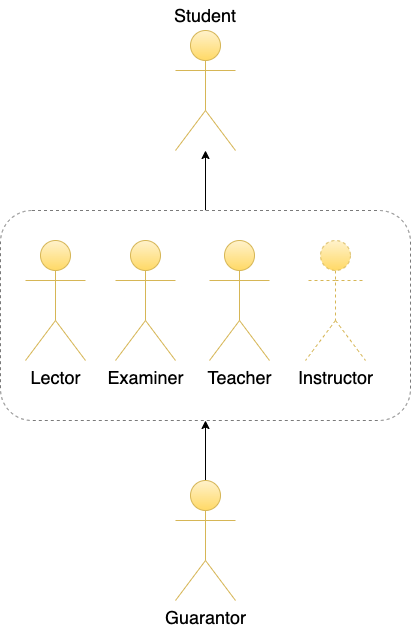
\includegraphics[scale=0.57]{../png/role.png}
\caption{Roles hierarchy}\label{picture:roles}
\end{figure}


\section{Permissions} modules and permissions... example of 

modules
\begin{itemize}
    \item Administration
    \item Semester Work
    \item Tests
    \item Connections
    \item Students score
    \item Users
\end{itemize}